
\documentclass[11pt]{exam} % https://www.ctan.org/pkg/exam?lang=en

\usepackage[lmargin=1.in,rmargin=1.in,tmargin=1.in,bmargin=1in]{geometry}
\usepackage{setspace}
\usepackage[pdftex]{graphicx}
\usepackage{titling}
\usepackage[
	pdfauthor={Brian Weinstein},
	pdftitle={Homework 1},
	bookmarks=true,
	colorlinks=true,
	linkcolor=blue,
	urlcolor=blue,
	citecolor=blue,
	pdftex,
	linktocpage=true
	]{hyperref}
\usepackage[textsize=tiny]{todonotes}
\usepackage{float}
\setlength\parindent{0pt}
\usepackage{lipsum}
\usepackage{amsmath}
\usepackage{caption}


\qformat{\textbf{Problem \thequestion: \thequestiontitle}\quad \hfill}


\pagestyle{headandfoot}
\runningheadrule
\firstpageheader{}{}{}
\runningheader{\theauthor}{\thetitle}{\thedate}
\firstpagefooter{}{\thepage}{}
\runningfooter{}{\thepage}{}


\usepackage{xcolor}
\usepackage{adjustbox}
\usepackage{verbatim}
\definecolor{shadecolor}{rgb}{.9, .9, .9}

\newenvironment{code}%
   {\par\noindent\adjustbox{margin=1ex,bgcolor=shadecolor,margin=0ex \medskipamount}\bgroup\minipage\linewidth\verbatim}%
   {\endverbatim\endminipage\egroup}

\newenvironment{codeSmall}%
   {\par\noindent\adjustbox{margin=1ex,bgcolor=shadecolor,margin=0ex \medskipamount}\bgroup\minipage\linewidth\verbatim\footnotesize}%
   {\endverbatim\endminipage\egroup}

\newcommand{\ramsey}{\href{http://www.statisticalsleuth.com/}{Ramsey }}



\begin{document}


\title{STAT W4201 001, Homework 9}
\author{Brian Weinstein (bmw2148)}
\date{Apr 13, 2016}
\maketitle

Code is attached here and also posted at \href{https://github.com/BrianWeinstein/advanced-data-analysis}{https://github.com/BrianWeinstein/advanced-data-analysis}. Where relevant, code snippets and output are are included in-line.

\begin{questions}


\titledquestion{\ramsey 20.12}

\textit{Duchenne Muscular Dystrophy (DMD) is a genetically transmitted disease, passed from a mother to her children. Doctors must rely on some kind of test to detect the presence of the disease. The data in Display 20.15 are levels of two enzymes in the blood, creatine kinase (CK) and hemopexin (H), for 38 known DMD carriers and 82 women who are not carriers. It is desired to use these data to obtain an equation for indicating whether a woman is a likely carrier.}

\begin{parts}

\part \textit{Make a scatterplot of $H$ versus $\log(CK)$; use one plotting symbol to represent the controls on the plot and another to represent the carriers. Does it appear from the plot that these enzymes might be useful predictors of whether a woman is a carrier?}

A coded scatterplot of $H$ vs $\log(CK)$ is shown in Figure \ref{fig:1a}. Based on the scatterplot, it does appear that these enzymes might be useful predictors of whether a woman is a carrier --- visually, at least, it looks like the carriers have higher levels of CK, and slightly higher levels of H.

\begin{codeSmall}
> mdData <- Sleuth3::ex2012
> mdData$Group <- relevel(mdData$Group, ref = "Control")
\end{codeSmall}

\begin{figure}[!h]
	\centering
	\captionsetup{width=0.8\textwidth}
	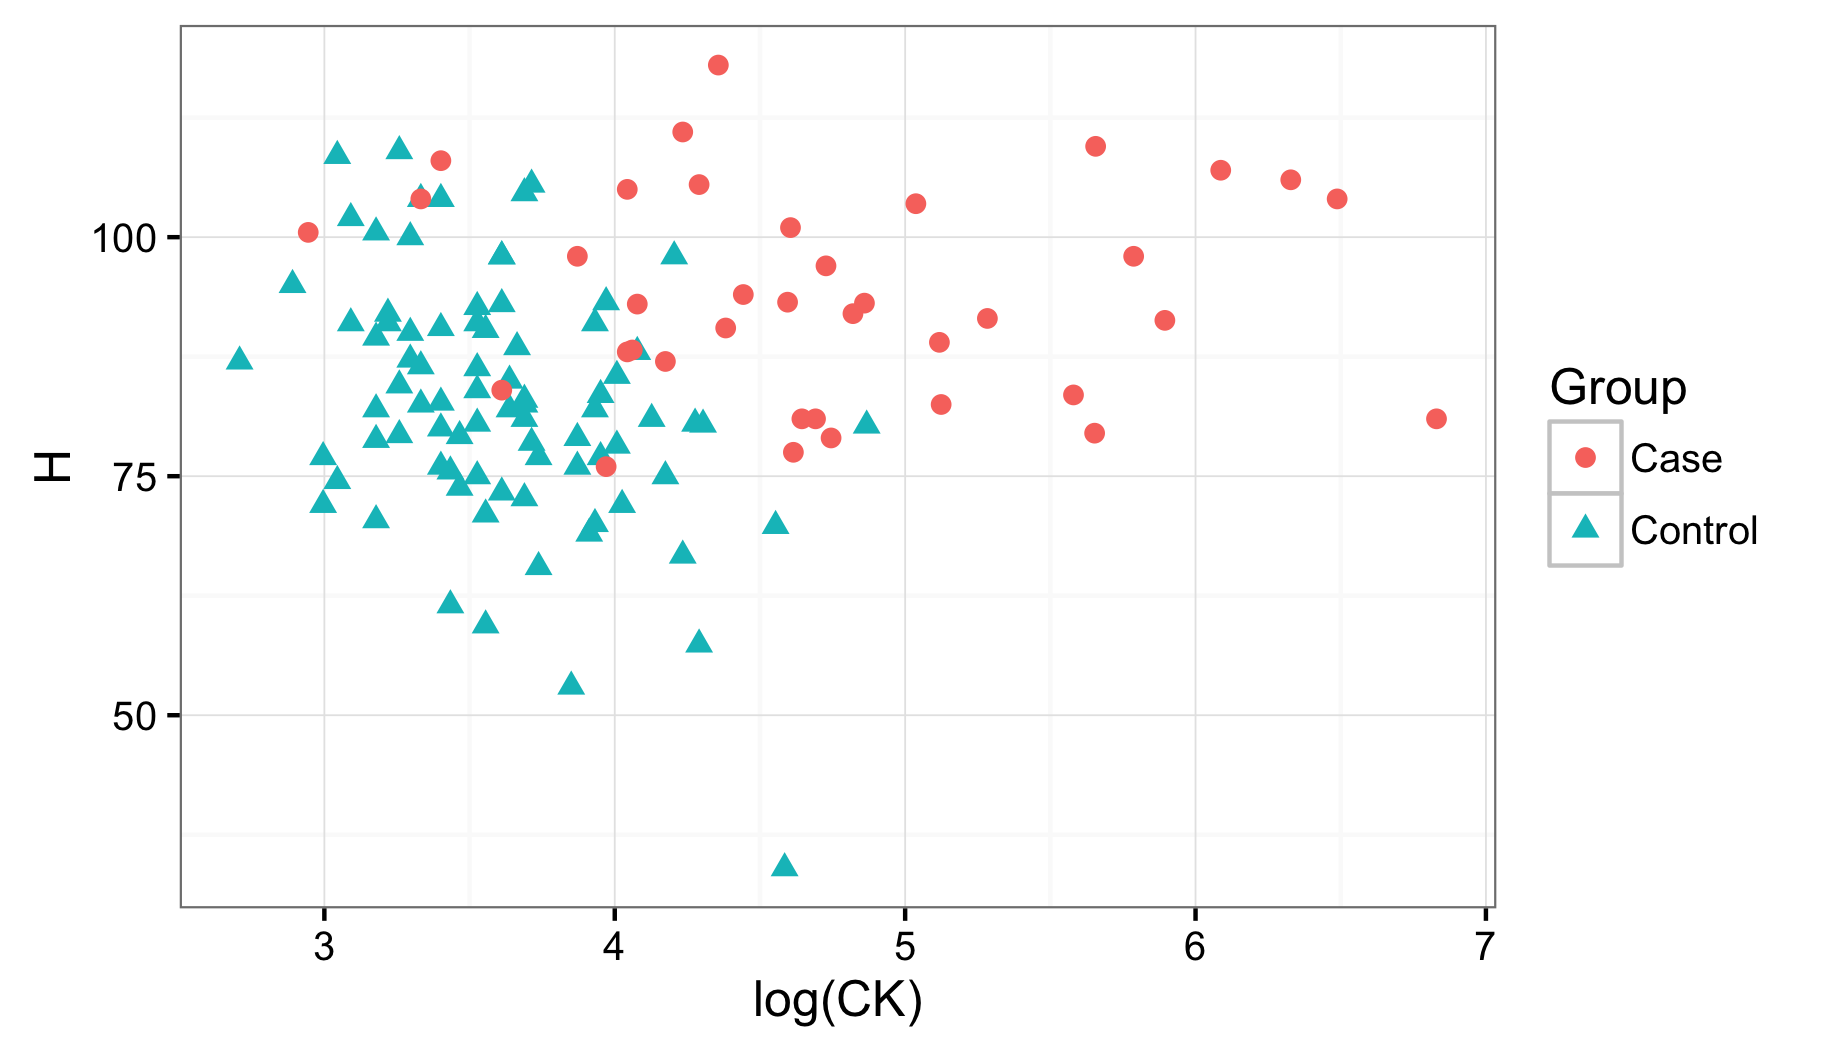
\includegraphics[width=4.25in]{1a.png}
	\caption{A coded scatterplot of $H$ vs $\log(CK)$.}
	\label{fig:1a}
\end{figure}



\part \textit{Fit the logistic regression of carrier on $CK$ and $CK$-squared. Does the $CK$-squared term significantly differ from 0? Next fit the logistic regression of carrier on $\log(CK)$ and $[\log(CK)]^2$. Does the squared term significantly differ from 0? Which scale (untransformed or log-transformed) seems more appropriate for $CK$?}

The logistic regression of carrier on $CK$ and $CK$-squared is shown below. The $CK$-squared term does not significantly differ from 0 (two-sided p-value 0.1219).

\begin{codeSmall}
> glm_1b1 <- glm(formula = Group ~ CK + I(CK^2),
+                data = mdData, family = binomial)
> summary(glm_1b1)$coefficients
                  Estimate    Std. Error   z value          Pr(>|z|)
(Intercept) -4.17746146864 0.72637612139 -5.751100 0.000000008866482
CK           0.05797905485 0.01299217478  4.462614 0.000008096600851
I(CK^2)     -0.00005054336 0.00003267841 -1.546690 0.121938045015287
\end{codeSmall}$

The logistic regression of carrier on $\log(CK)$ and $[\log(CK)]^2$ is shown below. The $[\log(CK)]^2$ term does not significantly differ from 0 (two-sided p-value 0.1737).

\begin{codeSmall}
> glm_1b2 <- glm(formula = Group ~ log(CK) + I(log(CK)^2),
+                data = mdData, family = binomial)
> summary(glm_1b2)$coefficients
              Estimate Std. Error    z value  Pr(>|z|)
(Intercept)   9.735313  16.297521  0.5973493 0.5502742
log(CK)      -8.516251   8.358066 -1.0189261 0.3082381
I(log(CK)^2)  1.445731   1.062746  1.3603736 0.1737117
\end{codeSmall}$

The log-transformed scale is more appropriate for $CK$, since it ranges over many orders of magnitude on the untransformed scale (from 15 to 925). A coded scatterplot of $H$ vs $CK$, shown in Figure \ref{fig:1b}, further illustrates the need for the transformation.

\begin{figure}[!h]
	\centering
	\captionsetup{width=0.8\textwidth}
	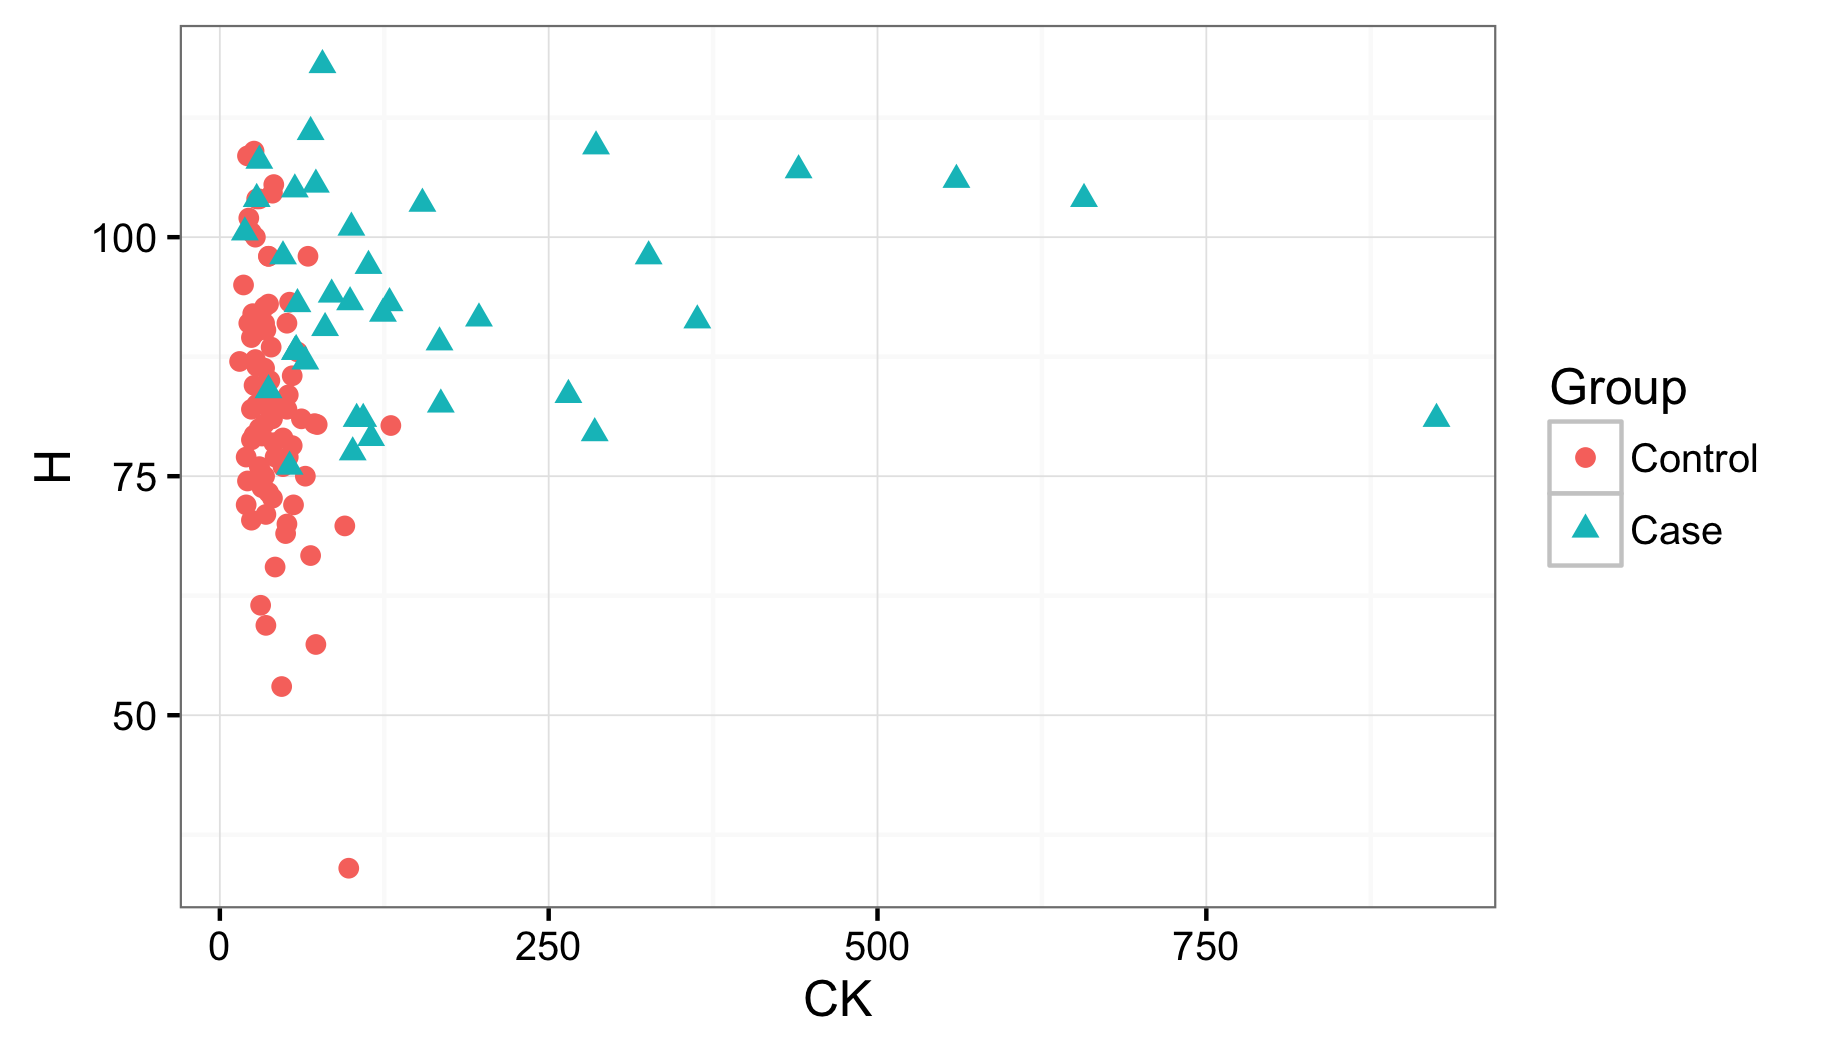
\includegraphics[width=4.25in]{1b.png}
	\caption{A coded scatterplot of $H$ vs $CK$.}
	\label{fig:1b}
\end{figure}



\part \textit{Fit the logistic regression of carrier on $\log(CK)$ and $H$. Report the coefficients and standard errors.}

The coefficients and standard errors in the logistic regression of carrier on $\log(CK)$ and $H$ is shown below.

\begin{codeSmall}
> glm_1c <- glm(formula = Group ~ log(CK) + H,
+                data = mdData, family = binomial)
> summary(glm_1c)$coefficients
               Estimate Std. Error   z value       Pr(>|z|)
(Intercept) -28.9134030 5.80016937 -4.984924 0.000000619862
log(CK)       4.0204252 0.82909534  4.849171 0.000001239784
H             0.1365189 0.03654202  3.735943 0.000187013358
\end{codeSmall}$



\part \textit{Carry out a drop-in-deviance test for the hypothesis that neither $\log(CK)$ nor $H$ are useful predictors of whether a woman is a carrier.}

We first fit a reduced model that includes only an intercept term.

\begin{codeSmall}
> glm_1d <- glm(formula = Group ~ 1,
+               data = mdData, family = binomial)
> summary(glm_1d)$coefficients
              Estimate Std. Error   z value      Pr(>|z|)
(Intercept) -0.7691331  0.1962419 -3.919311 0.00008880244
\end{codeSmall}$

We then compare the model from part (c) to this reduced model using a drop-in-deviance test (likelihood ratio test), testing the hypothesis that neither $\log(CK)$ nor $H$ are useful predictors of whether a woman is a carrier.

\begin{codeSmall}
> anova(glm_1c, glm_1d, test="LRT")
Analysis of Deviance Table

Model 1: Group ~ log(CK) + H
Model 2: Group ~ 1
  Resid. Df Resid. Dev Df Deviance  Pr(>Chi)    
1       117     61.992                          
2       119    149.840 -2  -87.847 < 2.2e-16 ***
---
Signif. codes:  0 ‘***’ 0.001 ‘**’ 0.01 ‘*’ 0.05 ‘.’ 0.1 ‘ ’ 1
\end{codeSmall}

There is overwhelming evidence that either (1) one of the variables or (2) both of the variables are useful predictors of whether a woman is a carrier of DMD (two-sided p-value $2.2 \times 10^{-16}$ from a drop-in-deviance test).


\part \textit{Typical values of $CK$ and $H$ are 80 and 85. Suppose that a suspected carrier has values of 300 and 100. What are the odds that she is a carrier relative to the odds that a woman with typical values (80 and 85) is a carrier?}

The odds of a woman being a carrier with values of 300 and 100 is 1575 times higher than the odds of a woman with values of 80 and 85.

\begin{codeSmall}
> # calculate odds and probability of having DMD at CK=80, H=85
> odds1 <- exp(predict(glm_1c, data.frame(CK=80, H=85)))[[1]] ; odds1
[1] 1.361127
> 1 / (1 + exp(-odds1))
[1] 0.7959428
> # calculate odds and probability of having DMD at CK=300, H=100
> odds2 <- exp(predict(glm_1c, data.frame(CK=300, H=100)))[[1]] ; odds2
[1] 2143.332
> 1 / (1 + exp(-odds2))
[1] 1
> # calculate the odds ratio
> odds2/odds1
[1] 1574.675
\end{codeSmall}


\end{parts}



\titledquestion{\ramsey 21.16}

\textit{Twenty tanks of rainbow trout embryos were exposed to one of five doses of Aflatoxicol for one hour. The data in Display 21.20 (from George Bailey and Jerry Hendricks) represent the numbers of fish in each tank and the numbers of these that had liver tumors after one year. Describe the relationship between dose of Aflatoxicol and odds of liver tumor. It is also of interest to determine the dose at which 50\% of the fish will get liver tumors. (Note: Tank effects are to be expected, meaning that tanks given the same dose may have slightly different  $\pi$’s. Thus, one should suspect extra-binomial variation.)}

A jittered scatterplot of logit(proportion of trout with liver tumors) vs log(Dose) is shown in Figure \ref{fig:2_scatter}. The scatterplot reveals a possible quadratic parameter.

\begin{figure}[!h]
	\centering
	\captionsetup{width=0.8\textwidth}
	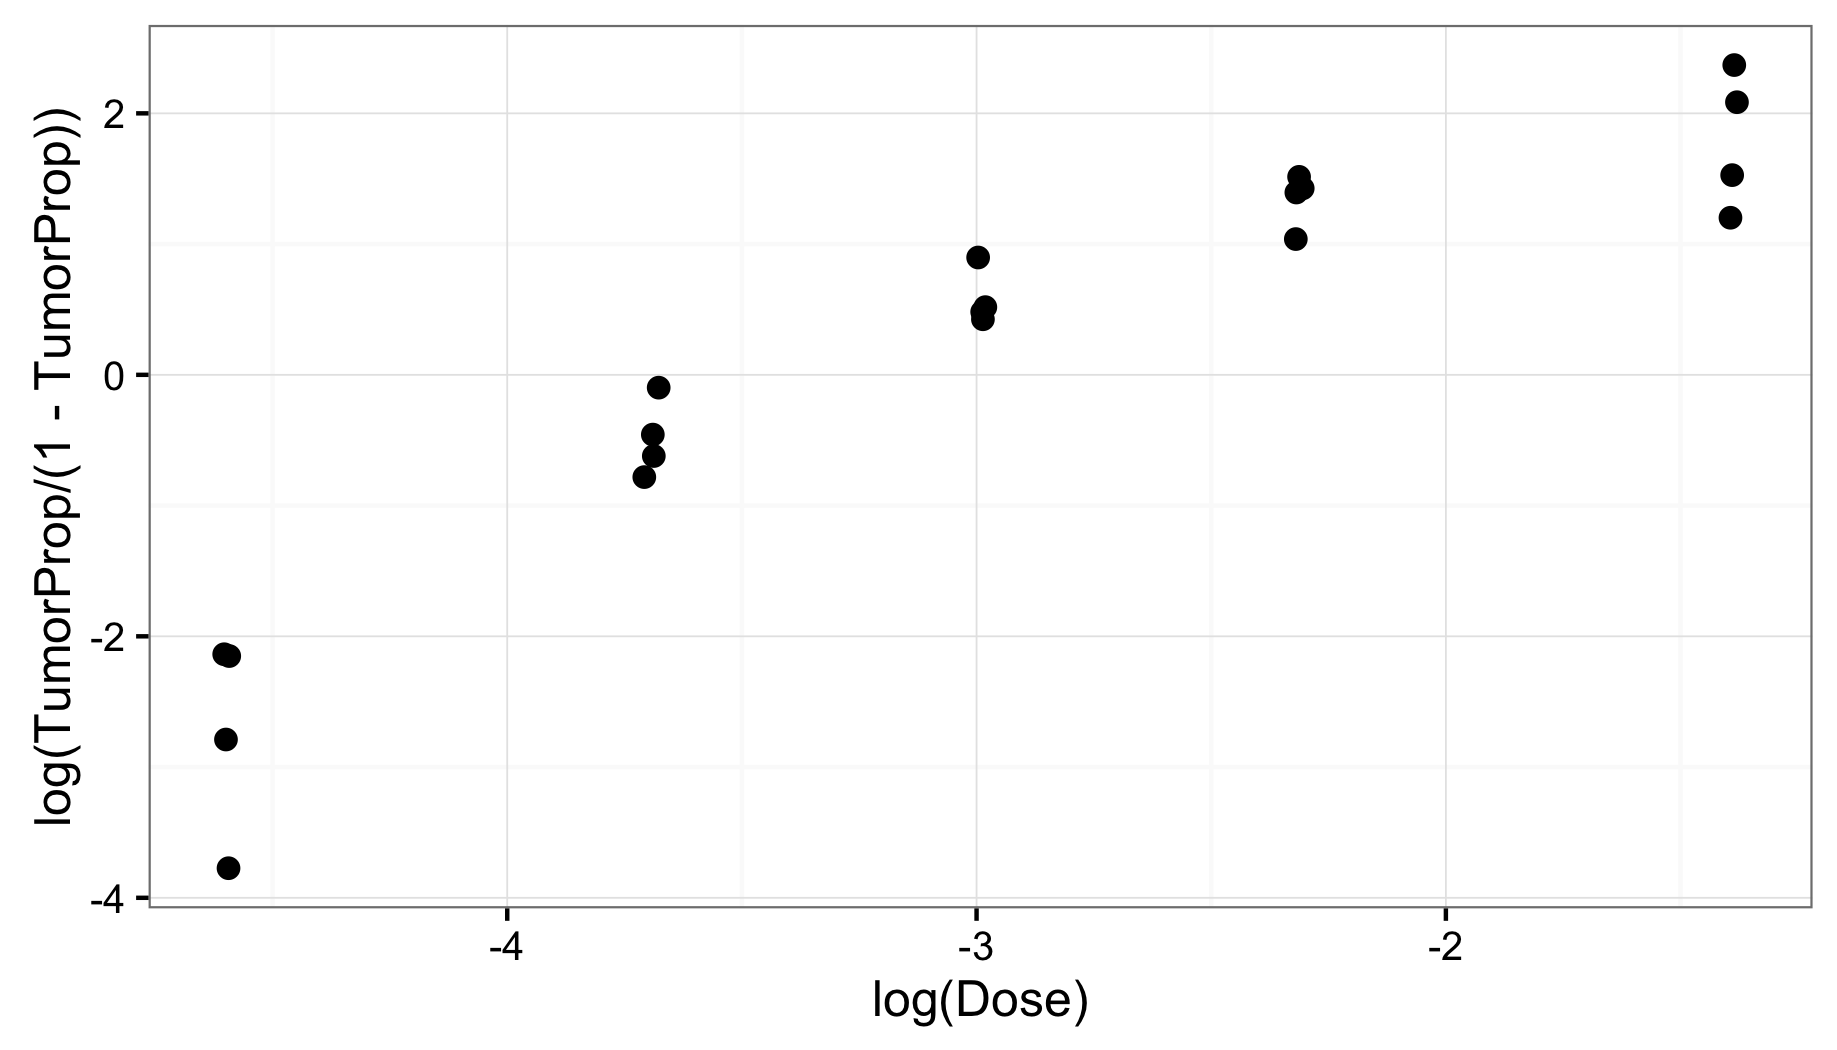
\includegraphics[width=4.25in]{2_scatter.png}
	\caption{A jittered scatterplot of logit(proportion of trout with liver tumors) vs log(Dose).}
	\label{fig:2_scatter}
\end{figure}


Based on the study design, there's no guarantee that, at each Dose, the $\pi$'s from each tank will be the same. As such, extra-binomial variation is suspected.

To test for extra-binomial variation, we first fit a rich model with both log(Dose) and [log(Dose)]$^2$ as explanatory variables, as shown below.

\begin{codeSmall}
> glm2 <- glm(formula = TumorProp ~ log(Dose) + I(log(Dose)^2),
+ data = troutData, family = binomial, weights = Total)
> summary(glm2)

Call:
glm(formula = TumorProp ~ log(Dose) + I(log(Dose)^2), family = binomial, 
    data = troutData, weights = Total)

Deviance Residuals: 
    Min       1Q   Median       3Q      Max  
-2.1349  -0.6860  -0.1067   1.0382   1.8863  

Coefficients:
               Estimate Std. Error z value Pr(>|z|)    
(Intercept)     1.02921    0.49343   2.086  0.03699 *  
log(Dose)      -1.03048    0.35743  -2.883  0.00394 ** 
I(log(Dose)^2) -0.39195    0.06136  -6.388 1.68e-10 ***
---
Signif. codes:  0 ‘***’ 0.001 ‘**’ 0.01 ‘*’ 0.05 ‘.’ 0.1 ‘ ’ 1

(Dispersion parameter for binomial family taken to be 1)

    Null deviance: 667.195  on 19  degrees of freedom
Residual deviance:  26.048  on 17  degrees of freedom
AIC: 119.45

Number of Fisher Scoring iterations: 4
\end{codeSmall}

The residual deviance of 26.048 on 17 degrees of freedom gives a p-value of 0.0736 from a goodness of fit test, as shown below. The p-value is low enough to indicate that the model is inadequate, and suggests the possible presence of extra-binomial variation.

\begin{codeSmall}
> pchisq(q = summary(glm2)$deviance, df = summary(glm2)$df.residual,
+        lower.tail = FALSE)
[1] 0.07358942
\end{codeSmall}

Examining a plot of the deviance residuals vs fitted values in Figure \ref{fig:2_devresid}, only one residual --- for the tank at Dose 0.010, where only 2 of the 89 fish had tumors --- is extreme. There's no pattern in the residual plot, so this likely isn't the cause of the low p-value from the goodness of fit test and can likely be ignored. We thus assume that cause of the low p-value is due to the presence of extra-binomial variation.

\begin{figure}[!h]
	\centering
	\captionsetup{width=0.8\textwidth}
	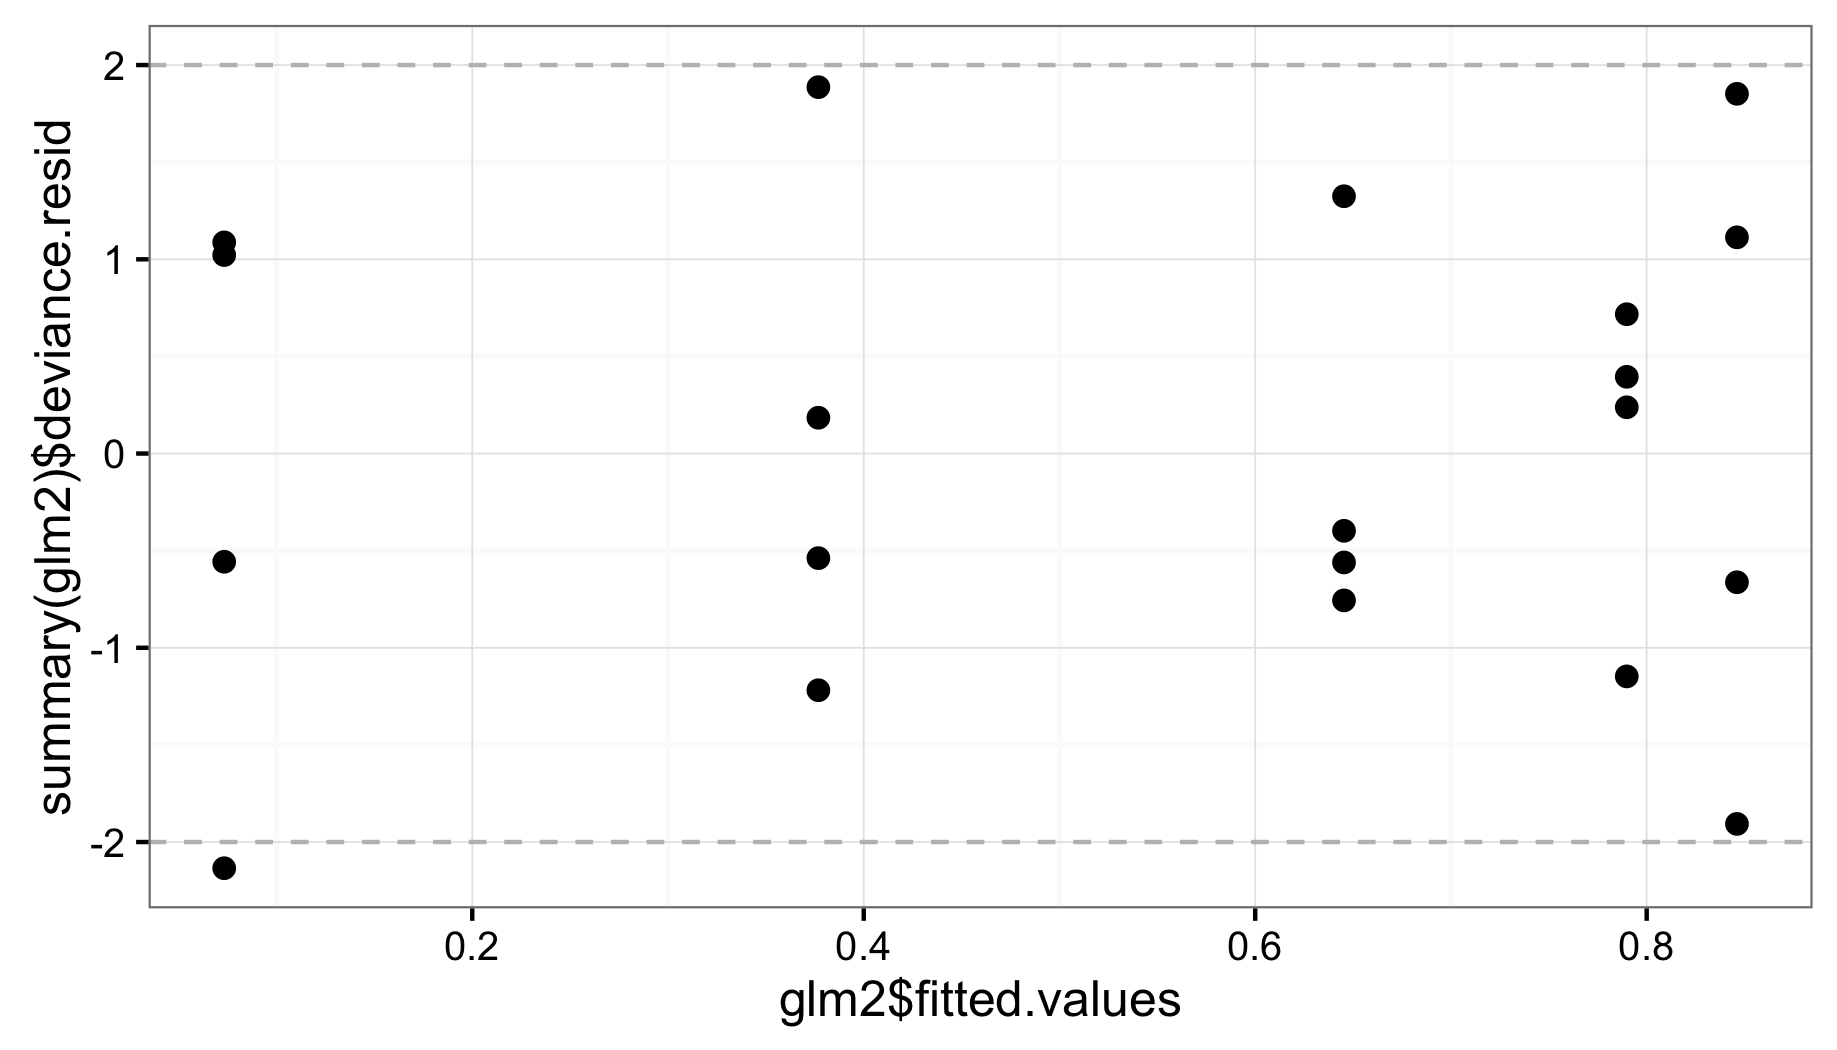
\includegraphics[width=4.25in]{2_devresid.png}
	\caption{Scatterplot of deviance residuals vs fitted values, for \texttt{glm2}.}
	\label{fig:2_devresid}
\end{figure}


Next, taking extra-binomial variation into account, we adjust the standard errors t-statistics, and associated p-values for the model estimates.

The dispersion parameter is estimated to be $\hat{\psi}=\frac{26.048}{17}=1.5322$, the quasi-likelihood standard error is $\text{sqrt}(\hat{\psi})$ times the maximum likelihood standard error, the t-value is the the estimate divided by the quasi-likelihood standard error, and the associated two-sided p-value (now based on the t distribution, with 17 degrees of freedom) is defined in the normal way. The computation, and  summary of the maximum-likelihood and quasi-likelihood statistics are shown below.

\begin{codeSmall}
> glm2QuasiSummary <- data.frame(summary(glm2)$coefficients) %>%
+   mutate(Term=row.names(.)) %>%
+   select(Term, Estimate, ML_StdError=Std..Error, ML_ZValue=z.value, ML_PValue=Pr...z..) %>%
+   mutate(QL_StdError=ML_StdError * sqrt(dispersion_param),
+          QL_TValue=Estimate/QL_StdError)
> glm2QuasiSummary$QL_PValue <- 2 * pt(q = -1 * abs(glm2QuasiSummary$QL_TValue),
+                                      df = as.integer(summary(glm2)$df.residual))
> glm2QuasiSummary[, -1] <- round(glm2QuasiSummary[, -1], 5)
> glm2QuasiSummary
            Term Estimate ML_StdError ML_ZValue ML_PValue QL_StdError QL_TValue QL_PValue
1    (Intercept)  1.02921     0.49343   2.08585   0.03699     0.61078   1.68508   0.11024
2      log(Dose) -1.03048     0.35743  -2.88306   0.00394     0.44243  -2.32911   0.03244
3 I(log(Dose)^2) -0.39195     0.06136  -6.38761   0.00000     0.07595  -5.16031   0.00008
\end{codeSmall}

The final model is thus:

\begin{codeSmall}
            Term Estimate QL_StdError QL_TValue QL_PValue
1    (Intercept)  1.02921     0.61078   1.68508   0.11024
2      log(Dose) -1.03048     0.44243  -2.32911   0.03244
3 I(log(Dose)^2) -0.39195     0.07595  -5.16031   0.00008
\end{codeSmall}

\todo{describe relationship between dose and odds}







\todo{find does at which 50 pct of fish get tumors}






\titledquestion{} % Problem 3

\textit{Suppose that a population of individuals is partitioned into sub-poplations or groups, $G_1$ and $G_2$. It may be helpful to think of $G_1$ in an epidemiological context as the carriers of a particular virus, comprising $100\pi_1$\% of the population, and $G_2$ as the non-carriers. Measurements $Z$ made on individuals have the following distributions in the two groups:
\begin{gather*}
G_1 \quad : \quad Z \sim N(\mu_1, \Sigma) \\
G_2 \quad : \quad Z \sim N(\mu_2, \Sigma)
\end{gather*}
Let $z$ be an observation made on an individual drawn at random from the combined population. The prior odds that the individual belongs to $G_1$ are $\pi_1/(1 - \pi_1)$. Show that the posterior odds given $z$ are
$$\frac{\pi_1}{1 - \pi_1} \exp(\alpha + \beta^T z )$$
and give the form of $\alpha$ and $\beta$.}




\end{questions}

\listoftodos

\end{document}